% LaTeX Midground Template: Boxed Content
% This template places the title and content inside a styled TikZ box.
% It requires TikZ, which should be included in the master document.

% Note: \documentclass, \usepackage, \begin{document}, \end{document}
% are provided by the master LaTeX document that includes this file.

\begin{center} % Center the entire box on the page
    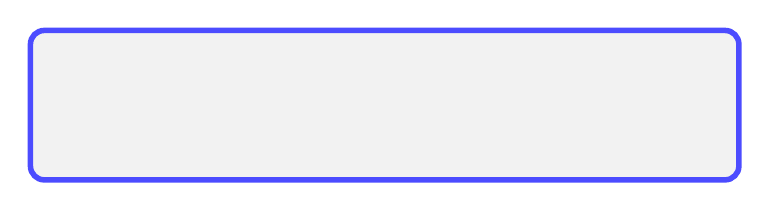
\begin{tikzpicture}
        % Define box properties
        \def\boxwidth{0.8\textwidth} % Box width relative to text width
        \def\boxfillcolor{gray!10}    % Light gray fill
        \def\boxbordercolor{blue!70}  % Blue border
        \def\boxborderwidth{2pt}
        \def\boxcornerradius{5pt}

        % Draw the main box node
        \node[
            draw=\boxbordercolor,
            fill=\boxfillcolor,
            line width=\boxborderwidth,
            rounded corners=\boxcornerradius,
            text width=\boxwidth - 2*\pgfkeysvalueof{/pgf/inner xsep} - 2*\pgfkeysvalueof{/pgf/inner ysep}, % Adjust text width for padding
            inner sep=10pt, % Padding inside the box
            align=left % Text alignment within the box
        ] (contentbox) {
            % Title inside the box
            % The %%TITLE%% placeholder will be replaced by the API 'title' parameter.
            \begin{center}
                \Large\bfseries %%TITLE%%
            \end{center}
            \vspace{1em} % Space after title

            % Content inside the box
            % The %%CONTENT%% placeholder will be replaced by the API 'content' parameter.
            %%CONTENT%%
        };
    \end{tikzpicture}
\end{center}

% --- Optional: Add more elements outside the box if needed ---
